\documentclass[conference]{IEEEtran}
\usepackage[T1]{fontenc}
\usepackage{amsmath,amssymb,booktabs,graphicx}
\usepackage[hidelinks]{hyperref}
\usepackage{microtype}
\title{Regime-Guided Forecasting Adaptation:\\Accuracy, Scale, and Baseline Fidelity}
\author{\IEEEauthorblockN{Author 1, Author 2}}
\begin{document}
\maketitle
\begin{abstract}
Recurring distributions offer opportunities to reuse forecasting models, but distributional similarity alone does not establish that a historical model remains useful. We study RG-TTA, a controller that combines a bounded checkpoint memory, observed-loss acceptance, similarity-dependent learning rates, and early stopping. An explicitly causal batch protocol evaluates four compact backbones on six real and eight synthetic streams, four horizons, and three seeds, yielding 4,704 policy results. Relative to fixed-step adaptation, RG-TTA obtains geometric mean MSE ratios of 0.950 on real streams and 0.919 on synthetic streams, with corresponding total-time ratios of 1.41 and 1.44. Focused experiments extend the study to 3.3--3.5 million-parameter attention models with head, adapter-plus-head, and full-model updates. Their mixed outcomes show that the preferred update scope depends on the backbone. Dependence-aware signatures do not improve consistently over simpler statistics. A separate six-run released-code DynaTTA/TAFAS comparison uses shared 6.4 million-parameter source checkpoints and a different evaluation protocol; it is not pooled with the batch results. These findings support a qualified accuracy--cost benefit for regime-guided adaptation, while exposing unresolved questions about retrieval attribution, baseline tuning, and generalization beyond the evaluated streams.
\end{abstract}
\begin{IEEEkeywords}
time-series forecasting, online adaptation, regime recurrence, causal evaluation
\end{IEEEkeywords}

\section{Introduction}
A deployed forecaster encounters changes in level, variance, seasonality, and relationships between variables. Updating on recent observations can reduce mismatch, but can also discard useful historical parameters or increase error. If distributions recur, a stored model may provide a useful initialization. The key difficulty is deciding whether similarity in observed data justifies transferring that model.

RG-TTA couples a distribution-indexed checkpoint memory with an observed-loss gate and a variable update rule. It is an empirical controller, not a guarantee that recurring marginals imply recurring predictive relationships. We evaluate three questions: (i) how its accuracy and cost compare with fixed adaptation under common forecast origins; (ii) whether its behavior persists with larger attention models and deeper updates; and (iii) whether richer regime signatures and changes in a dynamic baseline materially change the conclusions.

Our contributions are an evaluated combination of retrieval and adaptation controls, a causal batch comparison with explicit provenance for corrected runs, and focused evidence about its limitations. The main matrix contains 672 model--stream--horizon--seed settings and seven policies. Ninety-three additional settings examine scale, representation, and controller components. We separately run released DynaTTA code rather than treating a local learning-rate reimplementation as a faithful reproduction. We do not claim a new foundation model, a universally beneficial regime detector, or a convex optimization guarantee for neural adaptation.

\section{Related Work and Evaluation Scope}
TAFAS uses gated calibration modules and partially observed ground truth to adapt forecasting models~\cite{tafas}. DynaTTA introduces shift-dependent adaptation~\cite{dynatta}. PETSA investigates parameter-efficient calibration and dynamic gating~\cite{petsa}. Thus, adapters and dynamic learning rates alone are not sufficient novelty claims. The question examined here is whether a bounded memory with observed-loss acceptance improves a particular adaptation controller, and under which conditions.

The recent delay-aware audit of Fentazi \emph{et al.}~\cite{delay} emphasizes that a forecast's labels cannot be used before they become available and that source training and simple correction baselines can dominate adaptation comparisons. Our batch protocol respects observed-history boundaries, but differs from their dense, explicitly delayed evaluation. It does not evaluate additional label latency, nor compare with their closed-form correctors. These remain distinct questions rather than implied strengths of our study.

We use local implementations of iTransformer, PatchTST, DLinear, and a small GRU. The first three are motivated by inverted attention, patch-based modeling, and linear decomposition, respectively~\cite{itransformer,patchtst,dlinear}. Local architectural and preprocessing choices mean their scores should not be read as reproductions of the original backbone papers. The released-code comparison in Section~\ref{sec:official} uses its own upstream architecture and training recipe.

\section{Regime-Guided Controller}
\subsection{Observed History and Memory}
At origin $t$, the available history is $\mathcal H_t=\{(y_i,x_i):i\leq t\}$. The task is to issue $\hat y_{t+1:t+H}$ before observing these targets. Adaptation is supervised by previously observed labels; it is not label-free adaptation.

The memory stores at most five entries, evicting the oldest entry when full. Each entry contains a model state, a statistical signature, and the observed target samples used to compute that signature. The target signature comprises mean, standard deviation, skewness, excess kurtosis, and lag-one autocorrelation. The default multivariate signature appends covariate means and standard deviations. It therefore represents marginal information rather than general cross-variable dependence.

For a query and memory entry, similarity is
\begin{equation}
 s=0.3s_{\mathrm{KS}}+0.3s_{\mathrm{W}}+0.2s_{\mathrm{F}}+0.2s_{\sigma}.
\end{equation}
Here $s_{\mathrm{KS}}=1-D_{\mathrm{KS}}$, $s_{\mathrm{W}}=(1+W_1/R)^{-1}$, and $R$ is the larger within-sample target range, bounded below by a numerical constant. The feature score is $(1+\|f_q-f_m\|/a)^{-1}$, where $a$ is the mean of the two feature norms plus a small constant. The scale score is the ratio of the smaller to larger target standard deviation. We retrieve the highest-scoring entry. Most of the similarity weight remains target-based even when the feature vector is enriched.

\subsection{Acceptance and Gradient Updates}
A retrieved state is eligible when $s\geq0.75$. Let $\ell_t$ denote loss on sequences formed entirely from available history. We accept a candidate only if
\begin{equation}
 \ell_t(\theta_{\mathrm{candidate}})<0.70\ell_t(\theta_{\mathrm{current}}).
\end{equation}
The task loss is Smooth L1 with $\beta=1$, applied after clipping scaled targets and predictions to $[-5,5]$. If the gate rejects the candidate, we restore an independently cloned snapshot of the current weights. The gate measures current empirical fit, not future risk; it may reject useful transfer or accept harmful transfer under conditional shifts. Memory stores model states, not jointly versioned scaler states, so historical weights are evaluated under the current preprocessing state.

RG-TTA uses Adam with
\begin{equation}
 \alpha_t=3\!\times\!10^{-4}\,[1+0.67(1-s_t)].
\end{equation}
Updates stop after at most 25 gradient steps, with a minimum of five steps, relative-loss-improvement threshold 0.005, and patience three. The current loss is used both for acceptance and stopping; it is not an independent validation set. The adapted state is added to memory after the update. RG-EWC adds a diagonal-Fisher penalty with coefficient 400; RG-Dyna combines retrieval and stopping with the local dynamic learning-rate implementation.

Fixed-step TTA uses 20 steps at $3\times10^{-4}$. Head adaptation freezes the backbone of attention and recurrent models; DLinear's trainable linear projections have no analogous deep backbone. In the scale study, internal bottleneck adapters are updated together with the head, or all parameters are updated. We do not treat adapter-plus-head adaptation as adapter-only adaptation.

\subsection{Theoretical Scope}
Neural backbone, adapter, and full-model objectives need not be convex. A generic smooth-objective descent argument for exact gradient descent would not establish convergence of this Adam-based controller, whose objective and retrieved state change over time. Consequently, we make no theorem asserting that similarity increases safe learning rates or that the gate improves future forecasting error. The contribution and its limitations are evaluated empirically. This scope also avoids interpreting head freezing as evidence that the entire deployed loss is convex.

\section{Experimental Design}
\subsection{Causal Batch Matrix}
The real streams are ETTh1, ETTh2, ETTm1, ETTm2, Weather, and Exchange. We predict the supplied \texttt{OT} target using available numeric covariates. Eight univariate synthetic streams cover stable behavior, a trend break, slow drift, fast switching, recurring regimes, volatility shifts, shock recovery, and mixed regimes. Each synthetic condition is one fixed realization; the three seeds change training randomness, not stream generation.

For lookback $L=96$ and $H\in\{96,192,336,720\}$, the initial prefix length is $\max(720,L+H+100)$. We retain at most ten subsequent batches of 750 observations. After batch $B_j$ becomes observable, a policy updates and forecasts the first $H$ values of $B_{j+1}$. These targets are withheld until after the forecast is issued. This yields nine origins in most settings. Exchange has nine, eight, eight, and seven origins at the four respective horizons because its retained tail is shorter. The protocol evaluates a short initial stream segment, not the entire conventional benchmark test split.

All policies use the same target intervals within a setting. Forecast inputs end at the latest observed timestamp. Min--max preprocessing is fitted to observed history, and TTA-family scalers expand their ranges from newly observed data. Missing numeric values are forward-filled; inspection found no leading missing or sentinel value in the six archived real streams, so the loader's backward-fill fallback does not reach into their future. Horizon-specific initialization changes which timestamps are evaluated; horizons are reported separately in the detailed tables.

TTA-family policies use 15 initial epochs and chronological validation within the observed prefix. Each initial fit resets NumPy and PyTorch seeds. The main matrix does not archive a single shared source checkpoint per policy comparison, so matching seeds should not be equated with independently verified identical weights. Training randomness after initialization and CUDA numerical behavior can also produce small variations across repeated controls.

The always-retrain implementation uses 20 initial epochs and up to 30 epochs on accumulated observations per update. It has a separate training path, and its measured runtime includes an auxiliary partial-model branch even when the full model is selected for forecasting. It is an implementation-level accuracy reference, not a matched-training or optimized compute baseline. We do not interpret its runtime ratio as the intrinsic speed advantage of RG-TTA.

\subsection{Focused Reviewer Studies}
All focused studies use $H=96$ and seeds 0, 1, and 2. The scale study compares compact models with width-256, four-layer, eight-head attention configurations on ETTh1. It contrasts head-only, adapter-plus-head, and full updates. Total and adapted parameter counts are measured after model initialization. Peak CUDA allocation is recorded for the complete two-policy job, including initial training; it is not isolated adaptation memory.

The signature study compares target-only, marginal, and dependence-aware features on ETTh1, Weather, and CovShift. The dependence vector adds contemporaneous channel correlations, per-channel lag correlations at lags 1, 6, and 24, and a lag-one cross-channel matrix. It also log-compresses the marginal block and normalizes each block by the square root of its dimension. Thus, the contrast changes both information and feature scaling.

CovShift uses an autoregressive target and a covariate that alternates between positively and negatively correlated versions of that target. The marginal construction is approximately preserved while cross-variable association changes. The target's autoregressive dynamics remain unchanged, so this stress case does not ensure that changing covariates are necessary for optimal prediction. We do not infer general regime-detection accuracy from forecasting error alone.

Component studies remove retrieval, remove the loss acceptance gate while retaining the similarity threshold, fix the RG learning rate, or freeze both model and scaler updates. A separate sensitivity study varies the local Dyna-style EMA and warmup. Hyperparameters are fixed settings, not the outcome of an equal-budget validation search across all policies.

\subsection{Aggregation and Provenance}
We first average origin-level MSE within each run, then average the three seed results within each model--stream--horizon setting. A win means a strictly smaller seed-mean MSE; it does not mean statistical significance. Across heterogeneous streams, we summarize ratios by geometric means rather than averaging their raw MSEs. For ratios $r_i$, the aggregate is $\exp(N^{-1}\sum_i\log r_i)$. Real and synthetic streams are separated. Detailed tables retain MSE, MAE, sample standard deviation across seeds, and measured time for every setting. Seed variation is not a confidence interval over streams or temporally dependent forecast origins.

All experiments use RTX 4090 GPUs. Main-table time includes initial fitting, adaptation, and prediction, with CUDA synchronization. Corrected policies and unaffected baselines ran on different hosts of the same GPU type; exact hardware-normalized speed comparisons are therefore not claimed. The archived source and data hashes identify each execution source.

Two implementation failures were corrected before assembling the tables. Checkpoint rejection originally retained an aliased state; all three affected RG policies were rerun using cloned snapshots. DLinear's retraining optimizer originally received no parameters because layers were created lazily; all 168 DLinear retraining settings were rerun after a first-forward initialization fix. Failed outputs are excluded and successful replacement keys are checked against the planned matrix. Validation verifies archive checksums, unique experiment keys, seed coverage, finite errors, aggregation consistency, and equal causal target intervals across policies.

\section{Results}
\begin{table*}[t]
\centering
\caption{Main causal batch matrix. Columns 2--4 summarize 96 real-stream settings; columns 5--7 summarize 128 synthetic settings. Ratios are geometric means after averaging three seeds. Time is total measured pipeline time. Lower ratios are better; wins are descriptive. Retrain uses a different recipe and includes auxiliary training overhead.}
\label{tab:main}
\begin{tabular}{lrrrrrr}
\toprule
Policy & MSE/TTA & Wins & Time/TTA & MSE/TTA & Wins & Time/TTA \\
\midrule
TTA & 1.000 & -- & 1.00 & 1.000 & -- & 1.00 \\
EWC & 1.065 & 27/96 & 6.11 & 1.111 & 20/128 & 6.79 \\
Dyna-style & 1.177 & 22/96 & 1.03 & 1.165 & 32/128 & 1.04 \\
Retrain & 1.168 & 41/96 & 82.82 & 1.464 & 37/128 & 101.83 \\
RG-TTA & 0.950 & 61/96 & 1.41 & 0.919 & 85/128 & 1.44 \\
RG-EWC & 0.950 & 61/96 & 10.70 & 0.918 & 85/128 & 11.93 \\
RG-Dyna & 1.114 & 26/96 & 1.67 & 1.109 & 40/128 & 1.65 \\
\bottomrule
\end{tabular}

\end{table*}

\subsection{Accuracy and Measured Cost}
Table~\ref{tab:main} shows that RG-TTA reduces the geometric mean MSE ratio to 0.950 on real streams and 0.919 on synthetic streams relative to fixed-step TTA, winning 61/96 and 85/128 settings. Its corresponding time ratios are 1.41 and 1.44. Thus, the main evidence is an accuracy--cost tradeoff, not a simultaneous accuracy and runtime improvement.

When each controller is compared with its own base implementation, Table~\ref{tab:matched} shows gains for RG-EWC and RG-Dyna as well. However, RG-Dyna still has worse aggregate MSE than ordinary TTA in Table~\ref{tab:main}. Improving a weaker base does not establish superiority over the strongest simple baseline. RG-EWC has almost the same aggregate error ratio as RG-TTA relative to TTA, at substantially greater measured cost. The data do not establish EWC as a necessary component.

\begin{table}[t]
\centering
\caption{All 224 settings, each controller versus its own base: TTA, EWC, or local Dyna-style.}
\label{tab:matched}
\begin{tabular}{lrrr}
\toprule
Controller & MSE/base & Wins & Time/base \\
\midrule
RG-TTA & 0.932 & 146/224 & 1.43 \\
RG-EWC & 0.853 & 163/224 & 1.75 \\
RG-Dyna & 0.950 & 169/224 & 1.60 \\
\bottomrule
\end{tabular}

\end{table}

\begin{figure*}[t]
\centering
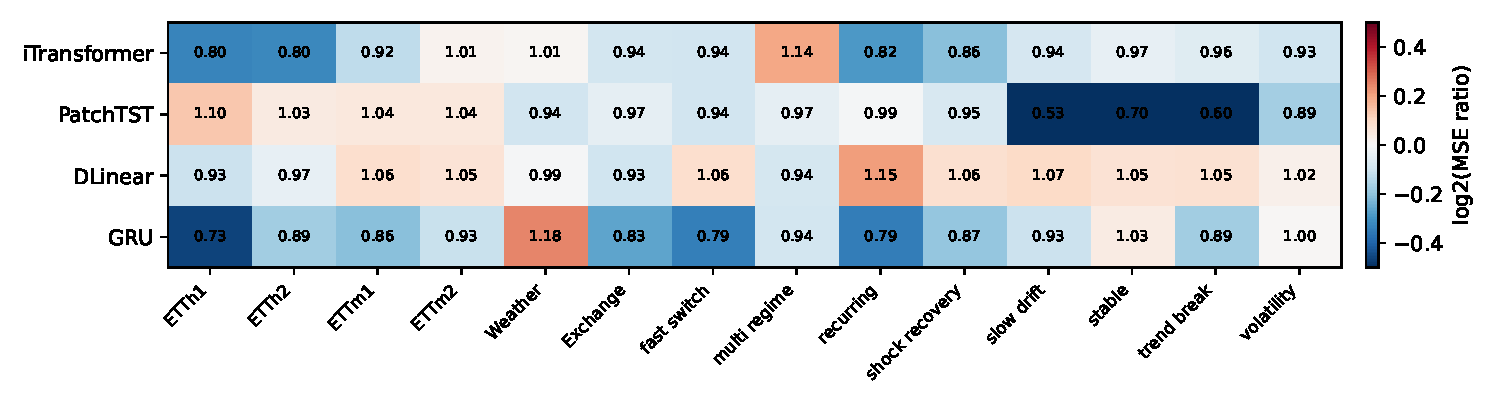
\includegraphics[width=.98\textwidth]{generated/rgtta_ratios.pdf}
\caption{RG-TTA/TTA MSE ratios, geometrically averaged over the four horizon-specific seed means. Values below one favor RG-TTA. All evaluated streams are shown; cells are descriptive summaries, not significance tests.}
\label{fig:ratios}
\end{figure*}

Figure~\ref{fig:ratios} preserves stream and backbone heterogeneity. Across all streams and horizons, RG-TTA/TTA ratios are 0.927 for iTransformer, 0.887 for PatchTST, 1.022 for DLinear, and 0.897 for GRU. In particular, the controller does not improve the aggregate DLinear result. A favorable overall ratio should not be used to conceal this failure case.

\subsection{Larger Models and Adaptation Depth}
\begin{table*}[t]
\centering
\caption{ETTh1, $H=96$, three seeds. MSE is mean $\pm$ sample SD. T/R denotes TTA/RG-TTA total time. Peak memory is the complete two-policy job, not adaptation-only memory. Adapter updates also include the output head.}
\label{tab:scale}
\small
\begin{tabular}{llrrrrrr}
\toprule
Backbone & Update scope & Total & Adapted & TTA MSE & RG MSE & Time T/R (s) & Peak MiB \\
\midrule
iTransformer & Compact/head & 123,040 & 6,240 & $35.08\pm3.33$ & $24.34\pm0.75$ & 4.05/3.65 & 51 \\
iTransformer & Larger/head & 3,299,616 & 24,672 & $30.41\pm1.70$ & $29.90\pm2.07$ & 5.71/5.45 & 174 \\
iTransformer & Larger/adapter+head & 3,335,520 & 60,576 & $22.77\pm1.23$ & $22.65\pm1.11$ & 9.29/9.76 & 442 \\
iTransformer & Larger/full & 3,299,616 & 3,299,616 & $25.40\pm1.02$ & $26.84\pm2.25$ & 8.44/8.24 & 663 \\
PatchTST & Compact/head & 191,602 & 67,680 & $182.22\pm2.81$ & $178.08\pm1.64$ & 4.51/4.46 & 284 \\
PatchTST & Larger/head & 3,469,362 & 270,432 & $128.46\pm19.36$ & $172.45\pm20.02$ & 12.36/10.54 & 1110 \\
PatchTST & Larger/adapter+head & 3,505,266 & 306,336 & $91.50\pm21.19$ & $115.33\pm54.84$ & 23.46/20.23 & 3951 \\
PatchTST & Larger/full & 3,469,362 & 3,469,362 & $78.24\pm5.64$ & $62.67\pm12.51$ & 26.67/31.07 & 6048 \\
\bottomrule
\end{tabular}

\end{table*}

Table~\ref{tab:scale} expands RG evaluation beyond compact backbones to 3.30--3.51 million parameters. On the larger iTransformer, adapter-plus-head RG-TTA achieves MSE 22.65, compared with 29.90 for head-only and 26.84 for full updates. Its advantage over adapter-plus-head TTA is small: 22.65 versus 22.77. On the larger PatchTST, full RG updates achieve 62.67 versus 78.24 for full TTA, whereas RG performs worse than TTA for both larger head-only and adapter-plus-head configurations. These contrasts demonstrate feasibility and sensitivity to update scope, not a universal preference for frozen backbones or adapters.

The largest peak allocation is approximately 6,048 MiB for the full PatchTST job. Memory measurements include training and both policies and therefore cannot quantify an adapter-only memory saving. The study covers one real stream and one horizon; it provides no foundation-model-scale or broad multivariate scalability guarantee.

\subsection{Regime Features and Component Attribution}
\begin{table}[t]
\centering
\caption{RG-TTA signature comparison, iTransformer, $H=96$; MSE mean $\pm$ seed SD.}
\label{tab:features}
\scriptsize
\begin{tabular}{lrrr}
\toprule
Signature & ETTh1 & Weather & CovShift \\
\midrule
Target 5D & $24.344\pm0.733$ & $117.892\pm29.722$ & $0.916\pm0.055$ \\
Marginal & $24.338\pm0.750$ & $117.945\pm29.541$ & $0.917\pm0.055$ \\
Dependence & $24.368\pm0.690$ & $118.036\pm29.736$ & $0.918\pm0.054$ \\
\bottomrule
\end{tabular}

\end{table}

Table~\ref{tab:features} provides no consistent advantage for the dependence-aware signature. On CovShift its MSE is 0.918 versus 0.916 for target-only features. On ETTh1, marginal features are slightly better, and on Weather target-only features are slightly better. The changes are small relative to seed variability. We therefore do not promote the richer signature as a validated accuracy contribution. The target-dominated similarity mixture and redundant autoregressive information in CovShift are plausible explanations to investigate, not established causes.

\begin{table}[t]
\centering
\caption{Component study, iTransformer, $H=96$. The full controller is the marginal-signature configuration.}
\label{tab:ablation}
\begin{tabular}{lrr}
\toprule
Variant & ETTh1 MSE & Weather MSE \\
\midrule
Frozen & $426.86\pm9.97$ & $88.87\pm4.04$ \\
Full RG-TTA & $24.34\pm0.75$ & $117.95\pm29.54$ \\
No retrieval & $25.66\pm1.55$ & $117.95\pm29.54$ \\
No loss gate & $25.18\pm0.95$ & $156.76\pm29.88$ \\
Constant RG LR & $27.75\pm1.61$ & $117.99\pm29.67$ \\
\bottomrule
\end{tabular}

\end{table}

The component results in Table~\ref{tab:ablation} are also context-dependent. Removing the loss gate increases Weather MSE from 117.95 to 156.76. Removing retrieval changes ETTh1 MSE from 24.34 to 25.66 but leaves Weather unchanged in the recorded means. Fixing the RG learning rate increases ETTh1 MSE to 27.75. The frozen control is worse on ETTh1 but better on Weather than the adapting variants. Because freezing suppresses scaler expansion as well as parameter updates, it measures the whole online pipeline change. These results support studying acceptance and learning-rate control, but do not isolate retrieval as the sole source of improvement. Early-stopping-only, tuned constant-rate, random-retrieval, and oracle-retrieval comparisons are not present.

\subsection{Baseline Sensitivity}
\begin{table}[t]
\centering
\caption{Local Dyna-style baseline sensitivity under the causal batch protocol; iTransformer, $H=96$. $w$ is warmup updates.}
\label{tab:sensitivity}
\begin{tabular}{lrr}
\toprule
Local baseline setting & ETTh1 & Weather \\
\midrule
$\eta=.1, w=60$ & $67.79\pm2.42$ & $133.10\pm31.73$ \\
$\eta=.7, w=60$ & $37.50\pm2.65$ & $99.60\pm32.27$ \\
$\eta=.1, w=96$ & $76.00\pm2.40$ & $143.04\pm30.12$ \\
\bottomrule
\end{tabular}

\end{table}

Changing the local EMA from 0.1 to 0.7 lowers Weather MSE from 133.10 to 99.60 (Table~\ref{tab:sensitivity}), below the approximately 118 obtained by RG-TTA in the same focused study. Changing warmup from 60 to 96 updates instead worsens the local baseline. This sensitivity limits any claim that RG-TTA dominates a well-tuned dynamic baseline. It is not an original-protocol reproduction, and selecting the favorable setting after observing test performance would not constitute fair validation tuning.

\section{Released-Code Baseline Check}\label{sec:official}
We separately execute the released DynaTTA adapter, copied byte-for-byte from commit \texttt{03c3cd9}, using the upstream TAFAS framework at \texttt{139bf98}. Device-portability substitutions leave CUDA behavior unchanged. This resolves the need to distinguish adapter reimplementation from released-code execution, but does not reproduce every published paper setting.

For ETTh1 and ETTh2 at $H=96$ and three seeds, we train fresh upstream iTransformer checkpoints with width 512, four layers, and a 30-epoch budget. Each model has 6,411,872 parameters. Frozen, TAFAS, and DynaTTA evaluations load the same validation-selected checkpoint within a seed. The saved checkpoint hash is checked against the completed training marker. TAFAS uses the upstream script's calibration settings (learning rate 0.001, zero weight decay, and initial gate 0.01); DynaTTA applies its released dynamic-rate configuration, including EMA 0.1 and horizon-based warmup.

\begin{table*}[t]
\centering
\caption{Released-code pipeline, standardized multivariate errors on 3,389 test windows per run. Three seeds, mean $\pm$ sample SD. Evaluation time excludes source training. This is a separate protocol; RG-TTA is not evaluated in this table.}
\label{tab:official}
\begin{tabular}{llrrr}
\toprule
Data & Policy & MSE & MAE & Eval. (s) \\
\midrule
ETTh1 & Frozen & $0.4515\pm0.0012$ & $0.4576\pm0.0010$ & 0.30 \\
ETTh1 & TAFAS & $0.4399\pm0.0023$ & $0.4515\pm0.0007$ & 3.34 \\
ETTh1 & DynaTTA & $0.4590\pm0.0039$ & $0.4697\pm0.0020$ & 14.44 \\
ETTh2 & Frozen & $0.2595\pm0.0097$ & $0.3436\pm0.0047$ & 0.30 \\
ETTh2 & TAFAS & $0.2563\pm0.0088$ & $0.3411\pm0.0042$ & 1.88 \\
ETTh2 & DynaTTA & $0.2804\pm0.0079$ & $0.3627\pm0.0015$ & 14.63 \\
\bottomrule
\end{tabular}

\end{table*}

Table~\ref{tab:official} reports all completed released-code comparisons. TAFAS improves on the frozen mean in both datasets; DynaTTA does not in this configuration. These outcomes do not establish that DynaTTA underperforms in its published benchmark, nor that RG-TTA outperforms the released method: RG-TTA is absent from this protocol. The upstream pipeline predicts all channels on standardized data and uses period-aware sliding evaluation, partial-ground-truth updates, and prediction adjustment. Its errors cannot be compared numerically with target-only, original-unit batch errors. The released implementation used here does not truncate evaluation to 500 windows. Full resolved configurations and per-window errors are retained, and no claim of exact numerical paper-table reproduction is made. An independent label-availability audit of the released prediction-adjustment logic remains necessary before calling this a causal protocol comparison.

\section{Limitations and Implications}
The strongest supported result is a modest aggregate improvement over a particular fixed-step baseline at additional cost. Six real streams, three training seeds, and a short initial segment do not establish broad deployment reliability. The larger-model study covers a narrow setting, richer signatures do not show consistent benefit, and Dyna-style sensitivity can reverse a ranking. Parameter-efficient adaptation, conditional retrieval, and dynamic rates already have substantial precedent; this work's claim is the evaluated controller combination and its documented boundaries.

Several comparisons remain necessary for stronger claims: matched source checkpoints and validation-only tuning budgets across batch policies; an optimized retraining path without unused work; simple naive and closed-form correction baselines; and an RG comparison inside the same independently audited released-code protocol. Larger-scale tests should add multiple streams and horizons rather than interpreting one favorable adaptation scope as general evidence. Retrieval should be tested separately from stopping and learning-rate changes, including negative-transfer cases and additional label delays. The present results do not justify a superiority or state-of-the-art claim over those untested settings.

\section{Conclusion}
RG-TTA can trade additional adaptation cost for lower aggregate forecasting error under the evaluated causal batch protocol. The completed matrix and focused studies also identify conditions in which adaptation, deeper updates, or richer regime representations fail to help. Separating protocol fidelity, model scale, and component attribution yields a more limited but reproducible account of regime-guided forecasting adaptation.

\section*{Use of AI Tools}
OpenAI Codex assisted with implementation, validation scripts, and manuscript drafting throughout this revision. The authors are responsible for checking the results, sources, and final claims. This disclosure does not represent independent scientific review.

\begin{thebibliography}{8}
\bibitem{tafas} H. Kim, S. Kim, J. Mok, and S. Yoon, ``Battling the non-stationarity in time series forecasting via test-time adaptation,'' AAAI, 2025. \url{https://arxiv.org/abs/2501.04970}.
\bibitem{dynatta} S. Grover and A. Etemad, ``Shift-aware test-time adaptation and benchmarking for time-series forecasting,'' 2025. Released code: \url{https://github.com/shivam-grover/DynaTTA}.
\bibitem{petsa} H. R. Medeiros, H. Sharifi-Noghabi, G. L. Oliveira, and S. Irandoust, ``Accurate parameter-efficient test-time adaptation for time series forecasting,'' 2025. \url{https://arxiv.org/abs/2506.23424}.
\bibitem{delay} M. R. Fentazi, M. Ameur, and A. Ksentini, ``Training on the future: A delay-aware audit of test-time adaptation for time-series forecasting,'' 2026. \url{https://arxiv.org/abs/2610.12232}.
\bibitem{itransformer} Y. Liu \emph{et al.}, ``iTransformer: Inverted transformers are effective for time series forecasting,'' ICLR, 2024.
\bibitem{patchtst} Y. Nie, N. H. Nguyen, P. Sinthong, and J. Kalagnanam, ``A time series is worth 64 words: Long-term forecasting with transformers,'' ICLR, 2023.
\bibitem{dlinear} A. Zeng, M. Chen, L. Zhang, and Q. Xu, ``Are transformers effective for time series forecasting?'' AAAI, vol. 37, pp. 11121--11128, 2023.
\end{thebibliography}
\end{document}
